\documentclass{article}
\usepackage[margin=0.6cm]{geometry}
\usepackage{tikz}
\usetikzlibrary{positioning}
\usepackage{booktabs}
\usepackage{amsmath}
\usepackage[table]{xcolor}
\usepackage{adjustbox}
\usepackage{multirow}
\pagestyle{empty}

\begin{document}

\begin{figure}[ht]
\centering
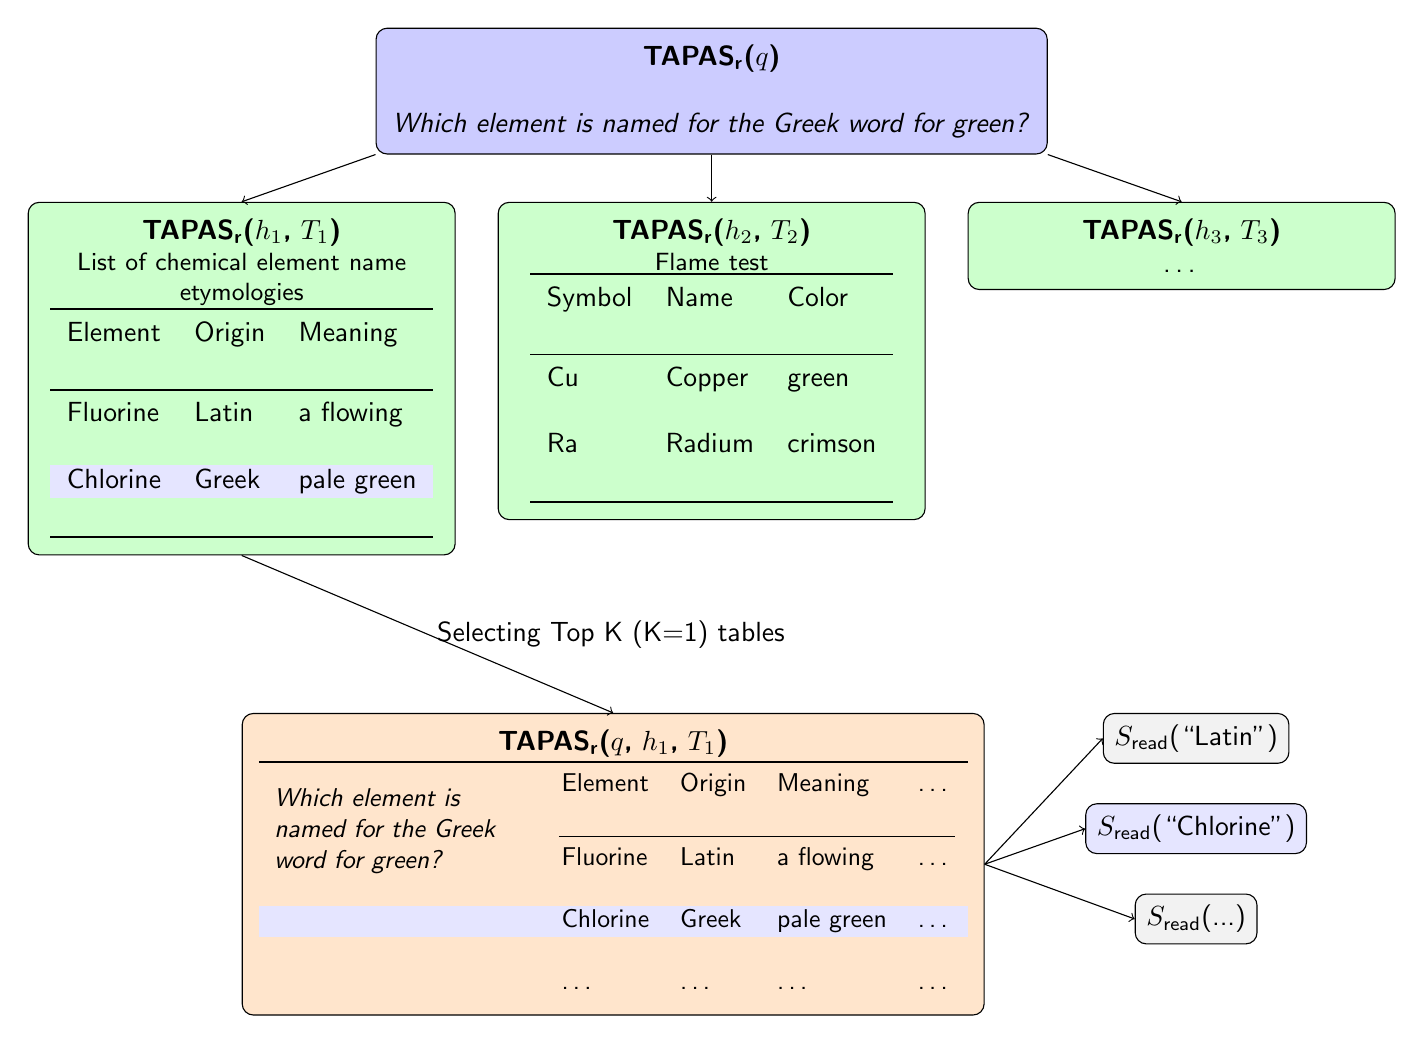
\begin{tikzpicture}[
  every node/.style={font=\sffamily},
  box/.style={draw, rounded corners, fill=#1!20, minimum width=4cm, inner sep=6pt, align=center},
  answerbox/.style={draw, rounded corners, fill=#1!10, inner sep=4pt, align=center},
  captionbox/.style={draw=none, fill=none, align=center},
  node distance=0.6cm and 0.7cm
  ]

% Question box
\node[box=blue, minimum width=8cm] (qbox) {
  \textbf{TAPAS\textsubscript{r}($q$)} \\\\
  \textit{Which element is named for the Greek word for green?}
};

% Left table
\node[box=green, text width=5cm, align=center, below left=of qbox, anchor=north, xshift=-1cm] (t1) {
    \parbox{\linewidth}{\centering 
    \textbf{TAPAS\textsubscript{r}($h_1$, $T_1$)} \\
    \small List of chemical element name etymologies}
  \begin{adjustbox}{max width=6cm}
  
  \begin{tabular}{lll}
  \toprule
  Element & Origin & Meaning \\\\
  \midrule
  Fluorine & Latin & a flowing \\\\
  \rowcolor{blue!10} Chlorine & Greek & pale green \\\\
  \bottomrule
  \end{tabular}
  \end{adjustbox}
};

% Middle table
\node[box=green, text width=5cm, align=center, below =of qbox] (t2) {
\parbox{\linewidth}{\centering 
    \textbf{TAPAS\textsubscript{r}($h_2$, $T_2$)} \\
    \small Flame test}
  \begin{adjustbox}{max width=5cm}
  \begin{tabular}{lll}
  \toprule
  Symbol & Name & Color \\\\
  \midrule
  Cu & Copper & green \\\\
  Ra & Radium & crimson \\\\
  \bottomrule
  \end{tabular}
  \end{adjustbox}
};

% Right table
\node[box=green, text width=5cm, align=center, below right=of qbox, anchor=north, xshift=1cm] (t3) {
  \parbox{\linewidth}{\centering 
    \textbf{TAPAS\textsubscript{r}($h_3$, $T_3$)} \\
    \dots}
  };


% Arrows from question to tables
\draw[->] (qbox.south west) -- (t1.north);
\draw[->] (qbox.south) -- (t2.north);
\draw[->] (qbox.south east) -- (t3.north);

% Final selected table
\node[box=orange, text width=9cm, align=center, below= 2cm of t1, anchor=north west] (final) {
  \textbf{TAPAS\textsubscript{r}($q$, $h_1$, $T_1$)} 
  \begin{adjustbox}{max width=9cm}
  \begin{tabular}{p{3.5cm}llll}
  \toprule
  \multirow{4}{=}{\textit{Which element is named for the Greek word for green?}}
  &Element & Origin & Meaning & \dots \\\\
  \cmidrule(lr){2-5}
  & Fluorine & Latin & a flowing & \dots \\\\
  \rowcolor{blue!10} 
  &Chlorine & Greek & pale green & \dots \\\\
  & \dots & \dots & \dots & \dots
  \end{tabular}
  \end{adjustbox}
};

% Answer boxes
\node[answerbox=gray, right=1.5cm of final.north east, anchor=north west] (a1) {$S_{\text{read}}$(``Latin'')};
\node[answerbox=blue, below=0.5cm of a1] (a2) {$S_{\text{read}}$(``Chlorine'')};
\node[answerbox=gray, below=0.5cm of a2] (a3) {$S_{\text{read}}$(...)};

% Arrows to answers
\draw[->] (t1.south) -- node[captionbox, right] {Selecting Top K (K=1) tables} (final.north);% arrow from selected table to final table
\draw[->] (final.east) -- (a1.west);
\draw[->] (final.east) -- (a2.west);
\draw[->] (final.east) -- (a3.west);

\end{tikzpicture}
\caption{An overview of the TAPAS approach. A dense table retriever scores the question against all tables and outputs the top $K$ tables ($K=1$ in this example), and a reader selects the answer from the top table.}
\end{figure}

\end{document}
